\tikzstyle{field}=[rectangle,draw=black,line width=1pt,align=center,font=\footnotesize,minimum height=1cm]
\linespread{0.8}

\scalebox{.66}{
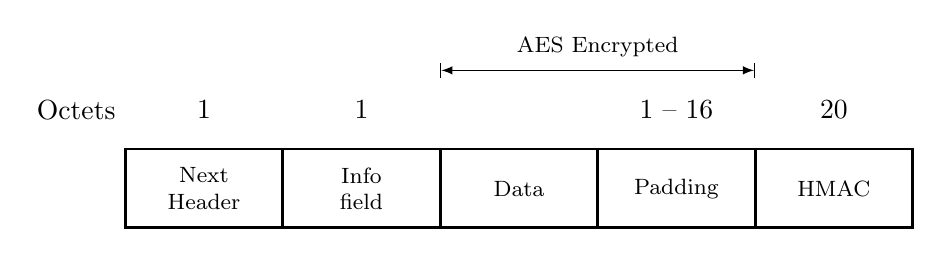
\begin{tikzpicture}[>=latex]
	%\draw (0,0) rectangle (2,1);
	\node[field,minimum width=2cm] at (0,0) {Next\\Header};
	\node[field,minimum width=2cm] at (2,0) {Info\\field};
	\node[field,minimum width=2cm] at (4,0) {Data};
	\node[field,minimum width=2cm] at (6,0) {Padding};
	\node[field,minimum width=2cm] at (8,0) {HMAC};

	\node at (5,1.8) {\footnotesize AES Encrypted};
	\draw[|<->|] (3,1.5) -- (7,1.5);

	% Bits
	\node[left] at (-1,1) {Octets};
	\node at (0,1) {1};
	\node at (2,1) {1};
	\node at (4,1) {};
	\node at (6,1) {1 -- 16};
	\node at (8,1) {20};
\end{tikzpicture}
}
